\documentclass[12pt]{article}
\usepackage[left=1cm, right=1cm, top=2cm,bottom=1.5cm]{geometry} 

\usepackage[parfill]{parskip}
\usepackage[utf8]{inputenc}
\usepackage[T2A]{fontenc}
\usepackage[russian]{babel}
\usepackage{enumitem}
\usepackage[normalem]{ulem}
\usepackage{amsfonts, amsmath, amsthm, amssymb, mathtools}
\usepackage{tikz}
\usepackage{tabularx}
\usepackage{hhline}

\usepackage{accents}
\usepackage{fancyhdr}
\pagestyle{fancy}
\renewcommand{\headrulewidth}{1.5pt}
\renewcommand{\footrulewidth}{1pt}

\usepackage{graphicx}
\usepackage[figurename=Рис.]{caption}
\usepackage{subcaption}
\usepackage{float}

%%Наименование папки откуда забирать изображения
\graphicspath{ {./images/} }

%%Изменение формата для ввода доказательства
\renewcommand{\proofname}{$\square$  \nopunct}
\renewcommand\qedsymbol{$\blacksquare$}

%%Изменение отступа на таблицах
\addto\captionsrussian{%
	\renewcommand{\proofname}{$\square$ \nopunct}%
}
%% Римские цифры
\newcommand{\RN}[1]{%
	\textup{\uppercase\expandafter{\romannumeral#1}}%
}

%% Для удобства записи
\newcommand{\MR}{\mathbb{R}}
\newcommand{\MQ}{\mathbb{Q}}
\newcommand{\MC}{\mathbb{C}}
\newcommand{\MI}{\mathrm{I}}
\newcommand{\MJ}{\mathrm{J}}
\newcommand{\MH}{\mathrm{H}}
\newcommand{\MT}{\mathrm{T}}
\newcommand{\MU}{\mathcal{U}}
\newcommand{\MV}{\mathcal{V}}
\newcommand{\VN}{\varnothing}
\newcommand{\VE}{\varepsilon}
\newcommand{\id}{\mathrm{id}}

\theoremstyle{definition}
\newtheorem{defn}{Опр:}
\newtheorem{rem}{Rm:}
\newtheorem{prop}{Утв.}
\newtheorem{exrc}{Упр.}
\newtheorem{lemma}{Лемма}
\newtheorem{theorem}{Теорема}
\newtheorem{corollary}{Следствие}

\newenvironment{cusdefn}[1]
{\renewcommand\thedefn{#1}\defn}
{\enddefn}

\DeclareRobustCommand{\divby}{%
	\mathrel{\text{\vbox{\baselineskip.65ex\lineskiplimit0pt\hbox{.}\hbox{.}\hbox{.}}}}%
}
%Короткий минус
\DeclareMathSymbol{\SMN}{\mathbin}{AMSa}{"39}
%Длинная шапка
\newcommand{\overbar}[1]{\mkern 1.5mu\overline{\mkern-1.5mu#1\mkern-1.5mu}\mkern 1.5mu}
%Функция знака
\DeclareMathOperator{\sgn}{sgn}

%Обозначение константы
\DeclareMathOperator{\const}{\text{const}}

%Интеграл в большом формате
\DeclareMathOperator{\dint}{\displaystyle\int}

\newcommand{\smallerrel}[1]{\mathrel{\mathpalette\smallerrelaux{#1}}}
\newcommand{\smallerrelaux}[2]{\raisebox{.1ex}{\scalebox{.75}{$#1#2$}}}

\newcommand{\smallin}{\smallerrel{\in}}
\newcommand{\smallnotin}{\smallerrel{\notin}}

\newcommand*{\medcap}{\mathbin{\scalebox{1.25}{\ensuremath{\cap}}}}%
\newcommand*{\medcup}{\mathbin{\scalebox{1.25}{\ensuremath{\cup}}}}%

%Скалярное произведение
\DeclarePairedDelimiterX{\inner}[2]{\langle}{\rangle}{#1, #2}

%Подпись символов снизу
\newcommand{\ubar}[1]{\underaccent{\bar}{#1}}

\newcommand*\circled[1]{\tikz[baseline=(char.base)]{
		\node[shape=circle,draw,inner sep=2pt] (char) {#1};}}


\begin{document}
\lhead{Линейная алгебра}
\chead{Мануйлов В.М.}
\rhead{Лекция - 3}
\section*{Записи векторов в координатах определенного базиса}
Пусть $e_1,\dotsc, e_n$ - базис в $V, \, x \in V, \, x^1, \dotsc, x^n \in \mathbb{K}$ - координаты $x$ в этом базисе $\Rightarrow$ 
$$x = x^ie_u = x^1e_1 + \dotsc + x^ne_n$$
Если $\widetilde{e}_1, \dotsc, \widetilde{e}_n$ - другой базис в $V \Rightarrow$ удобнее записывать так: 
$$
	\forall i, \, \widetilde{e}_i = c_i^j e_j = c_i^1 e_1 + \dotsc + c_i^n e_n
$$
Тогда: $x = x^i e_i = \widetilde{x}^k \widetilde{e}_k = \widetilde{x}^k c_k^j e_j \Rightarrow$ каждая координата выразится следующим образом: 
$$
	x^j = \widetilde{x}^k c_k^j = \widetilde{x}^1 c_1^j + \dotsc + \widetilde{x}^n c_n^j
$$

\section*{Изоморфизм в линейных пространствах}
Пусть $V, \, W$ - линейные пространства над полем $\mathbb{K}$.
\begin{defn}
	Отображение $f \colon V \to W$ называется \uwave{изоморфизмом}, если:
	\begin{enumerate}[label ={(\arabic*)}]
		\item $f$ - взаимно однозначно;
		\item $f$ - сохраняет структуру линейного пространства: 
		\begin{enumerate}[label ={\arabic*)}]
			\item $f(a + b) = f(a) + f(b), \, \forall a,b \in V$;
			\item $f(\lambda a) = \lambda{\cdot}f(a),\, \forall \lambda \in \mathbb{K}, \, \forall a\in V$;
		\end{enumerate}
	\end{enumerate}
\end{defn}

\textbf{Пример}: Если $W = V$, то $\id \colon V \to V, \, \id{(a)} = a, \, \forall a \in V$ - изоморфизм.
\begin{figure}[H]
	\centering
	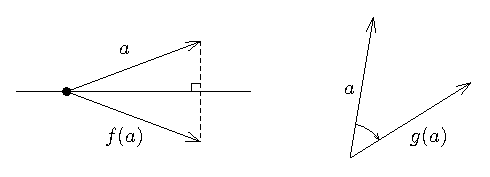
\includegraphics[width=0.45\textwidth]{3_1.eps}
	\caption{Зеркальное отражение $f(a)$. Поворот всех векторов $g(a)$.}
	\label{3_1}
\end{figure}
\textbf{Пример}: $f(a)$ - отражение, $f(f(a)) = a \Rightarrow f$ - изоморфизм.

\textbf{Пример}: $g(a)$ - поворот всех векторов, также изоморфизм.

\textbf{Пример}: $f\colon V \to W, \, f(a) = 0, \, \forall a \in V$ - не изоморфизм (нарушается взаимная однозначность).

\begin{defn}
	Линейные пространства $V$ и $W$ - \uwave{изоморфны}, если $\exists$ изоморфизм $f \colon V \to W$.
\end{defn}

\uline{\textbf{Обозначение}}: $V$ изоморфно $W \Leftrightarrow V \simeq W$.

Только что показали, что $V \simeq V, \, \forall \, V$ - линейное пространство (рефлексивность).
Очень похоже на отношение эквивалентности.

\newpage
\section*{Изоморфизм, как отношение эквивалентности}
Отношение эквивалентности обладает следующими свойствами:
\begin{enumerate}[label ={(\arabic*)}]
	\item $V \sim V, \, \forall\, V$ - линейное пространство (рефлексивность);
	\item Если $V$ эквивалентно $W$, то $W$ эквивалентно $V$ (симметричность);
	\item Если $V$ эквивалентно $W$, $W$ эквивалентно $U$, то $V$ эквивалентно $U$ (транзитивность);
\end{enumerate}
Если есть соотношения $(1)-(3)$ между объектами (отношение эквивалентности) $\Rightarrow$ можем разбивать объекты на классы эквивалентности.

\begin{lemma}
	Изоморфизм является симметричным и транзитивным.
\end{lemma}
\begin{proof}\hfill\\
	(\textbf{Симметричность}): Пусть $f \colon V \to W$ - изоморфизм, $f$ - взаимно однозначное $\Rightarrow \exists$ обратное к $f$ отображение $g \colon W \to V$ и тоже взаимно однозначное. 
	Тогда:
	\begin{enumerate}[label ={(\arabic*)}]
		\item $f(g(x+y)) = x+y \wedge f(g(x) + g(y)) = f(g(x)) + f(g(y)) = x + y \Rightarrow g(x+y) = g(x) + g(y)$;
		\item $f(g(\lambda x)) = \lambda x, \, f(\lambda g(x)) = \lambda f(g(x)) = \lambda x \Rightarrow g(\lambda x) = \lambda g(x)$;
	\end{enumerate}	

	(\textbf{Транзитивность}): Пусть $f\colon V \to W, \, h\colon W \to U$ - изоморфизмы. $h \circ f \colon V \to U$. Так как $f,h$ - взаимно однозначны, то $h \circ f$ - взаимно однозначная функция. $(h \circ f)(a) = h(f(a))$ и структура линейного пространства сохраняется:
	\begin{enumerate}[label ={(\arabic*)}]
		\item $h(f(x+y)) = h(f(x) + f(y)) = h(f(x)) + h(f(y))$;
		\item $h(f(\lambda x)) = h(\lambda f(x)) = \lambda h(f(x))$;
	\end{enumerate}
\end{proof}
Таким образом можно поделить линейные пространства на классы эквивалентностей.

\begin{lemma}
	Пусть $e_1,\dotsc, e_n$ - базис в $V$, $f\colon V \to W$ - изоморфизм, тогда $f(e_1),\dotsc, f(e_n)$ - базис в $W$.
\end{lemma}
\begin{proof}\hfill\\
	\textbf{(Линейная независимость)}: Рассмотрим следующую линейную комбинацию:
	$$
		\lambda_1 f(e_1) + \dotsc + \lambda_n f(e_n) = 0 \Leftrightarrow f(\lambda_1 e_1 + \dotsc + \lambda_n e_n) = 0
	$$
	Знаем, что $f(0) = 0$, так как сохраняется структура линейного пространства $\Rightarrow$ по взаимной однозначности:
	
	$$
		\lambda_1 e_1 + \dotsc + \lambda_n e_n = 0 \Rightarrow \forall \lambda_i = 0,\, i = \overline{1,n}
	$$
	
	\textbf{(Максимальность)}: Пусть $x \in W$, тогда $\exists \, a \in V \colon f(a) = x$ (по взаимной однозначности). 
	$$
		a = a_1 e_1 + \dotsc + a_n e_n \Rightarrow f(a) = f(a_1 e_1 + \dotsc + a_n e_n) = a_1 f(e_1) + \dotsc + a_n f(e_n) = x 
	$$
	Таким образом, любой элемент из $W$ можно представить как линейную коммбинацию элементов из $f(e_1),\dotsc, f(e_n)$.
\end{proof}
\newpage
\begin{corollary}
	Пусть $n = \dim{V},\, m = \dim{W}$, если $V \simeq W$, то $n = m$.
\end{corollary}
\begin{proof}
	Если $n \neq m$, то количество элементов в базисах разное $\Rightarrow$ противоречие с леммой.
\end{proof}

\begin{lemma}
	Пусть $\dim{V} = n$, тогда $V \simeq \mathbb{K}_n$ - линейное пространство строк длины $n$.
\end{lemma}
\begin{proof}
	Пусть $f \colon V \to \mathbb{K}_n$. Выберем в $V$ базис $e_1,\dotsc, e_n$ и возьмем элемент $a \in V,\, a = a_1 e_1 + \dotsc + a_n e_n$. Определим функцию $f(a) \coloneqq (a_1, \dotsc, a_n) \in \mathbb{K}_n$. Проверим, что она - изоморфизм:
	\begin{enumerate}[label ={(\arabic*)}]
		\item $f$ - взаимно однозначная:
		\begin{enumerate}[label ={\arabic*)}]
			\item \uline{Инъективность}: $f(a) = f(b) \Rightarrow a = b$ - очевидно;
			\item \uline{Сюръективность}: $\forall (a_1, \dotsc, a_n) \in \mathbb{K}_n, \, \exists \, a \in V \colon f(a) = (a_1, \dotsc, a_n)$, где $a = a_1 e_1 + \dotsc + a_n e_n$;
		\end{enumerate}
		Таким образом функция $f$ взаимно однозначна;
		\item $f$ сохраняет структуру линейного пространства:
		\begin{enumerate}[label ={\arabic*)}]
			\item Пусть $a = a_1 e_1 + \dotsc + a_n e_n, \, b = b_1 e_1 + \dotsc + b_n e_n$, тогда:
			$$
			a + b = (a_1 + b_1) e_1 + \dotsc + (a_n + b_n)e_n \Rightarrow 
			$$	
			$$
			\Rightarrow f(a+b) = (a_1 + b_1 , \dotsc , a_n + b_n) = f(a) + f(b) = (a_1, \dotsc , a_n) + (b_1, \dotsc, b_n) = (a_1 + b_1, \dotsc, a_n + b_n)
			$$
			\item Пусть $a = a_1 e_1 + \dotsc + a_n e_n, \, \lambda \in \mathbb{K}$, тогда:
			$$
				f(\lambda a) = (\lambda a_1, \dotsc, \lambda a_n) = \lambda (a_1, \dotsc, a_n) = \lambda f(a)
			$$	
		\end{enumerate}
		Таким образом, функция $f$ сохраняет структуру линейного пространства;
	\end{enumerate}
	И в результате $f$ - изоморфизм.
\end{proof}
\begin{corollary}
	Если $\dim{V} = \dim{W}$, то $V \simeq W$.
\end{corollary}
\begin{proof}
	По лемме $V \simeq \mathbb{K}_n, \, W \simeq \mathbb{K}_n \Rightarrow$ по транзитивности и симметричности $V \simeq \mathbb{K}_n \simeq W \Rightarrow V \simeq W$.
\end{proof}

\newpage
\section*{Двойственное пространство и линейные функции}
Пусть дано поле $\mathbb{K}$ и линейное пространство $V$ над ним.
\begin{defn}
	Отображение $l \colon V \to \mathbb{K}$ называется \uwave{линейной функцией}, если:
	\begin{enumerate}[label ={(\arabic*)}]
		\item $l(a+b) = l(a) + l(b), \, \forall a,b \in V$;
		\item $l(\lambda {\cdot} a) = \lambda {\cdot} l(a),\, \forall a \in V, \, \forall \lambda \in \mathbb{K}$;
	\end{enumerate}
\end{defn}

\textbf{Пример}: $V = \MR_n, \, x \in \MR_n, \, x = (x_1,\dotsc, x_n)$, тогда
\begin{itemize}
	\item $l(x) = x_1$ - линейная функция;
	\item $l(x) = x_1 + 1$ - не линейная функция;
	\item $l(x) = x_1 + \dotsc + x_n$ - линейная функция;
	\item $l(x) = 1$ - не линейная функция;
	\item $l(x) = 0$ - линейная функция;
	\item $l(x) = x_1^2 + \dotsc + x_n^2$ - не линейная;
\end{itemize}

$V$ - произвольное линейное пространство с базисом $e_1, \dotsc, e_n$, $a = a_1 e_1 + \dotsc + a_n e_n$, пусть $l_1$ и $l_2$ - произвольные линейные функции на $V$. Определим их сумму и умножение на скаляр, как:
\begin{enumerate}[label ={(\arabic*)}]
	\item $(l_1 + l_2)(a) \coloneqq l_1(a) + l_2(a)$ - линейная функция;
	\item $(\lambda {\cdot} l_1)(a) \coloneqq \lambda {\cdot} l_1(a))$ - линейная функция;
\end{enumerate}
Таким образом множество линейных функций образуют \uline{линейное пространство}.

\begin{defn}
	Множество линейных функций на $V$ со структурой указанной выше, образует линейное пространство, называемое \uwave{двойственным} к $V$ пространством, которое обозначим $V^\prime$.
\end{defn}
\begin{defn}
	Пусть $e_1,\dotsc, e_n$ - базис в $V$, $l$ - линейная функция. \uwave{Координатами} $l$ в этом базисе называются числа $l_1 = l(e_1), \dotsc, l_n = l(e_n)$.
\end{defn}
\begin{lemma}
	Пусть $l,h \in V^\prime$, если $l \neq h$, то $(l_1,\dotsc, l_n) \neq (h_1,\dotsc, h_n)$.
\end{lemma}
\begin{proof}
	(От противного) Пусть $l \neq h$, но $(l_1,\dotsc, l_n) = (h_1, \dotsc, h_n) \Rightarrow$ пусть $a \in V \Rightarrow l(a) = a_1 l_1 \dotsc + a_n l_n = $\\
	$= a_1{\cdot}l(e_1) + \dotsc + a_n {\cdot}l(e_n)$, $h(a) = a_1 h_1 + \dotsc + a_n h_n \Rightarrow h(a) = l(a), \, \forall a \in V \Rightarrow$ противоречие.
\end{proof}

\begin{lemma}
	$\forall l_1, \dotsc, l_n \in \mathbb{K}, \, \exists \, l \in V^\prime \colon l \mapsto (l_1,\dotsc, l_n)$.
\end{lemma}
\begin{proof}
	Есть набор $l_1,\dotsc, l_n \in \mathbb{K} \Rightarrow \forall a \in V, \, \exists \, l(a) = l_1{\cdot}a_1 + \dotsc + l_n{\cdot}a_n$ - линейная функция $\in V^\prime$.
\end{proof}

\begin{lemma}
	Сопоставление $l \mapsto (l_1,\dotsc, l_n)$ - взаимно однозначное, задает изоморфизм $V^\prime \simeq \mathbb{K}_n$.
\end{lemma}
\begin{proof}
	По лемме выше функция - линейная и взаимно однозначная $\Rightarrow$ это изоморфизм.
\end{proof}

Пусть $e_1, \dotsc, e_n$ базис в $V$. Рассмотрим следующие линейные функции $\VE^1, \dotsc, \VE^n \in V^\prime$, определяемые, как:
$$
	\VE^i(e_j) = \begin{cases} 1, & i = j\\ 0, & i \neq j \end{cases} \Rightarrow (\overset{1}{0}, \dotsc, \overset{i-1}{0}, \overset{i}{1}, \overset{i+1}{0},\dotsc, \overset{n}{0})\text{ - координаты }\VE^i
$$
Таким образом, мы получим $n$ линейных функций, которые линейно независимы.
\begin{proof}
	Рассмотрим функциональное равенство: $\lambda_1 \VE^1 + \dotsc + \lambda_n \VE^n = 0 \Rightarrow$ тогда:
	$$
		\lambda_1 \VE^1(e_i) + \dotsc + \lambda_i \VE^i(e_i) + \dotsc + \lambda_n \VE^n(e_i) = \lambda_i \VE^i(e_i) = \lambda_i = 0, \, \forall i = \overline{1,n}
	$$
	Таким образом, линейные функции $\VE^i$ - линейно независимы.
\end{proof}

Зная, что $\dim{V} = \dim{V^\prime} =n$ и $\VE^1,\dotsc, \VE^n$ - линейно независимы и этот набор - максимален $\Rightarrow$ получим двойственный к $e_1, \dotsc, e_n$ базис.

\begin{lemma}
	$\tilde{\VE}^i = d_j^i \VE^j$, где $d_j^i$ - элементы матрицы $D = C^{-1}$.
\end{lemma}
\begin{proof}
	Пусть в $V$ два базиса $e_1, \dotsc, e_n; \, \tilde{e}_1, \dotsc, \tilde{e}_n$ и пусть $C$ - это матрица перехода от $(e)$ к $(\tilde{e}) \Rightarrow \tilde{e}_i = c_i^j e_j$. Пусть тогда $\VE^1, \dotsc, \VE^n$ - двойственный к $(e)$, а $\tilde{\VE}^1, \dotsc, \tilde{\VE}^n$ - двойственна к $(\tilde{e})$.
	
	Пусть $\tilde{\VE}^i = d_j^i \VE^j \Rightarrow \tilde{\VE}^i(\tilde{e}_k) = \tilde{\VE}^i(c_k^je_j) = d_p^i \VE^p(c_k^je_j) = d_p^i c_k^j\VE^p(e_j) = \displaystyle \sum\limits_{j,p = 1}^n d_p^i c_k^j \VE^p(e_j) = \displaystyle \sum\limits_{j= 1}^n d_j^i c_k^j = d_j^i c_k^j$. Таким образом получили:
	$$
		\tilde{\VE}^i(\tilde{e}_k) = d_j^i c_k^j = \begin{cases} 1, & i = k \\ 0, & i \neq k \end{cases} \Rightarrow 
		C = 
		\begin{pmatrix} 
			c_1^1 & \dotsc & c_n^1\\ 
			\vdots & \ddots & \vdots \\ 
			c_1^n & \dotsc & c_n^n
		\end{pmatrix}, \, 
		D = 
		\begin{pmatrix} 
			d_1^1 & \dotsc & d_n^1\\ 
			\vdots & \ddots & \vdots \\ 
			d_1^n & \dotsc & d_n^n
		\end{pmatrix}, \, 
		(DC)_k^i = \begin{cases} 1, & i = k \\ 0, & i \neq k \end{cases}
	$$
	
	Таким образом, получим $DC = E \Rightarrow D = C^{-1}$.
\end{proof}


\end{document}